\documentclass[a4paper,11pt]{article}

\usepackage{textalpha}
\usepackage{multirow}
\usepackage{amssymb}
\usepackage{graphicx}
\usepackage{caption}
\usepackage{makecell}

\title{1\textsuperscript{η} Υποχρεωτική Εργασία Στο Μάθημα της Αριθμητικής Ανάλυσης}
\author{Ονοματεπώνυμο: Βίκτωρ Κυρτσούδης \\ ΑΕΜ: 4143}
\date{}

\boldmath
\begin{document}
\maketitle
\begin{flushleft}

Όλα τα προγράμματα για την επίλυση των ασκήσεων δημιουργήθηκαν σε Matlab.

\section*{Άσκηση 1}
\begin{figure}[ht]
    \caption*{Γραφική παράσταση των $f(x) = e^{sin^3x}+x^6-2x^4-x^3-1$ και \textbf{f'}}
    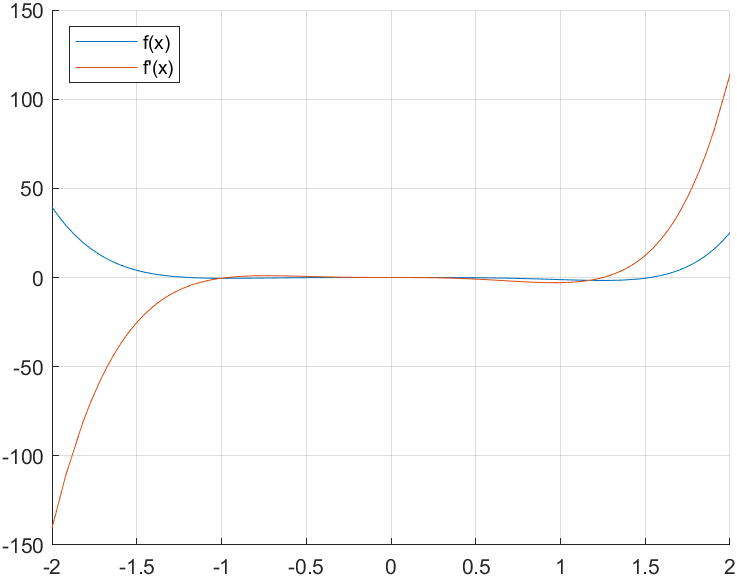
\includegraphics[width=\textwidth]{ex1plot.png}
\end{figure}

Από το γράφημα παρατηρούμε ότι:
\begin{enumerate}
    \item Η f φαίνεται να έχει ρίζες κοντά στα $x_1=-1$, $x_2=0$ και $x_3=1.5$.
    \item Η f' έχει ρίζα στο 0.
\end{enumerate}

Για τον υπολογισμό των ριζών δημιουργήθηκαν τα αρχεία ex1.m, bisection.m, newton.m και secant.m \newline

\textbf{Στο ex1} ορίζεται μία συμβολική συνάρτηση f με τον αντίστοιχο τύπο, κατασκευάζεται το παραπάνω γράφημα και στην συνέχεια καλούνται με τη σειρά οι τρεις συναρτήσεις για να υπολογίσουν την κάθε ρίζα και των αριθμό των επαναλήψεων που χρειάζονται για να τις προσεγγίσουν. Τα αποτελέσματα για κάθε μέθοδο αποθηκεύονται στους πίνακες 
\begin{itemize}
    \item bisectionRoots
    \item newtonRoots
    \item secantRoots
\end{itemize}

    
    
\begin{table}[h]
    \centering
    \begin{tabular}{|c|c|c|c|}
        \hline
        \multirow{2}{*}{Μέθοδος} & -1.1976 & 0.0000 & 1.5301 \\ \cline{2-4}  & \multicolumn{3}{c|}{Επαναλήψεις} \\
        \hline
        Bisection & 18 & - & 18 \\ \hline
        Newton & 8 & 36 & 7 \\  \hline
        Secant & 14 & 55 & 10 \\ \hline
    \end{tabular}
\end{table}

\subsection*{Διχοτόμηση}
Η συνάρτηση bisection υλοποιεί την μέθοδο της Διχοτόμησης και δέχεται την συνάρτηση $f$, το μέγιστο επιτρεπόμενο σφάλμα και τα ακρά του διαστήματος στο οποίο θα γίνει η αναζήτηση. Αφού υπολογίσει τον ελάχιστο αριθμο των αναγκαίων επαναλήψεων με τον τύπο 
$N > \frac{\ln{\frac{b-a}{\epsilon}}}{\ln{2}}$ 
ελέγχει αν το μέσο του διαστήματος είναι ρίζα της $f$ και αν ναι σταματάει και επιστρέφει τα αντίστοιχα αποτελέσματα. Αν δεν είναι αποφασίζει αν θα αντικαταστήσει το αριστερό ή το δεξί άκρο του διαστήματος με το μέσο δεδομένου ότι μετά την αντικατάσταση πρέπει να ισχύει: $f(a)f(b)<0$. Και επαναλαμβάνει μέχρι να βρει την ρίζα ή να φτάσει τις $N$ επαναλήψεις. \newline
Χρησιμοποιούμε την μέθοδο της διχοτόμησης μόνο για την αναζήτηση των ριζών κοντά στο -1 και στο 1.5 γιατί κοντά στο 0 δεν υπάρχει διάστημα $[a,b]$ με $a<0$ και $b>0$ που να ισχύει $f(a)f(b)<0$ \newline

\subsection*{Newton-Raphson}
Η συνάρτηση newton υλοποιεί την μέθοδο Newton-Raphson και δέχεται την συνάρτηση $f$, το μέγιστο επιτρεπόμενο σφάλμα και το αρχικό σημείο $x_0$. Αρχικά υπολογίζει την νέα προσέγγιση με τον επαναληπτικό τύπο $x_{n+1} = x_n-\frac{f(x_n)}{f'(x_n)}$ και την διαφορά των προσεγγίσεων. Μετά ξεκινάει η επαναληπτική διαδικασία κατά την οποία ελέγχει αν η διαφορά είναι μεγαλύτερη του μέγιστου επιτρεπόμενου σφάλματος. Αν δεν είναι τερματίζει και επιστρέφει τα αποτελέσματα. Αν είναι υπολογίζει την νέα προσέγγιση και διαφορά. Αν η καινούρια διαφορά των τελευταίων προσεγγίσεων είναι μεγαλύτερη από την προηγούμενη τότε σημαίνει ότι δεν συγκλίνει οπότε σταματάει και επιστρέφει $NaN$ στην προσέγγιση και $0$ στις επαναλήψεις.\newline
Παρόλο που στο 0 δεν υπάρχει διάστημα που να ικανοποιεί τις συνθήκες του θεωρήματος ύπαρξης μοναδικής ρίζας (δηλ. $f'(x),f''(x)\neq0$ για κάθε $x\in[a,b]$ και $f(a)f(b)<0$) η Newton-Raphson επιστρέφει τα σωστά αποτελέσματα.
\newline

\subsection*{Τέμνουσα}
Η συνάρτηση secant υλοποιεί την μέθοδο της Τέμνουσας και δέχεται την συνάρτηση $f$, το μέγιστο επιτρεπόμενο σφάλμα και τις αρχικές προσεγγίσεις $x_0$ και $x_1$. Μέχρι η διαφορά των δύο τελευταίων προσεγγίσεων να γίνει μικρότερη του σφάλματος επαναλαμβάνει την εξής διαδικασία: υπολογίζει την νέα προσέγγιση με βάση τις προηγούμενες δύο χρησιμοποιώντας τον τύπο $x_{n+1} = x_n-\frac{f(x_n)(x_n-x_{n-1})}{f(x_n)-f(x_{n-1})}$ και κάνει ξανά την σύγκριση. Στο τέλος επιστρέφει τα αποτελέσματα. \newline\newline


Οι επαναλήψεις που χρειάζεται η Διχοτόμηση στις δύο ρίζες είναι σχεδόν διπλάσιες από της Newton-Raphson. Ενώ της μεθόδου της Τέμνουσας βρίσκονται ανάμεσα.
Επίσης επειδή το 0 είναι ρίζα και της $f'$ (από το γράφημα) προκύπει ότι σε αντίθεση με τις ρίζες -1.1976 και 1.5301 η Newton-Raphson δεν συγκλίνει τετραγωνικά στο 0 γι' αυτό και χρειάζονται τόσες παραπάνω επαναλήψεις. Αντίστοιχα και για την Τέμνουσα.


\newpage

\section*{Άσκηση 2}

Για την επίλυση των ζητουμένων στο διάστημα $[0,3]$ πάνω στην συνάρτηση
$$f(x) = $$ $$94cos^3x-24cosx+177sin^2x-108sin^4x-72cos^3x*sin^2x-65$$
δημιουργήθηκαν τα αρχεία ex2.m, modifiedBisection, modifiedNewton και modifiedSecant.

\subsection*{modifiedBisection}
 Η συνάρτηση modifiedBisection υλοποιεί μια τροποποιημένη μέθοδο της διχοτόμησης η οποία αντί να επιλέγει το μέσο του διαστήματος σαν νέα προσέγγιση επιλέγει τυχαία έναν αριθμό μέσα από αύτο. Αυτό σημαίνει ότι το διάστημα δεν μειώνεται με σταθερό ρυθμό κι έτσι δεν μπορούμε να γνωρίζουμε απ' την αρχή πόσες επαναλήψεις χρειάζονται για την εύρεση της προσέγγισης με αποδεκτό σφάλμα για αυτό και η νέα τερματική συνθήκη είναι η διαφορά των δύο τελευταίων προσεγγίσεων να είναι μικρότερη του μέγιστου αποδεκτού σφάλματος.
\newline

\subsection*{modifiedNewton}
Η συνάρτηση modifiedNewton υλοποιεί μια τροποποιημένη μέθοδο Newton-Raphson η οποία κάνει ακριβώς ότι και η απλή μέθοδος Newton αλλά η συνάρτηση $\phi$ έχει τον τύπο $$x_{n+1} = x_n-\frac{1}{\frac{f'(x_n)}{f(x_n)}-\frac{1}{2}\frac{f''(x_n)}{f'(x_n)}}$$
\newline

\subsection*{modifiedSecant}
Η συνάρτηση modifiedSecant υλοποιεί μια τροποποιημένη μέθοδο της Τέμνουσας η οποία μοιάζει με την απλή μέθοδο Τέμνουσας με την διαφορά ότι η συνάρτηση $\phi$ δεν βρίσκει το σημείο στο οποίο τέμνει τον άξονα $x'x$ η ευθεία που περνάει από τις δύο τελευταίες προσεγγίσεις αλλά η παραβολή που περνάει από τις τρεις τελευταίες και έχει τον τύπο: 
$$x_{n+3} = x_{n+2} - \frac{r(r-q)(x_{n+2}-x_{n+1})+(1-r)s(x_{n+2}-x_n)}{(q-1)(r-1)(s-1)}$$
όπου $r = \frac{f(x_{n+2})}{f(x_{n+1})}$, $q = \frac{f(x_n)}{f(x_{n+1})}$ και $s = \frac{f(x_{n+2})}{f(x_n)}$.
\newline

\subsection*{2.1}

\textbf{Στο ex2} ορίζεται πάλι μία συμβολική συνάρτηση f και όπως και στην 1\textsuperscript{η} άσκηση καλούμε τις 3 συναρτήσεις για να επιστρέψουν την προσέγγιση στην οποία καταλήγουν και τις επαναλήψεις που χρειάστηκαν. Αυτό γίνεται και με τις τρεις συναρτήσεις της 1\textsuperscript{ης} άσκησης και τα αποτελέσματα αποθηκεύονται αντίστοιχα στους πίνακες: 
\begin{itemize}
    \item modifiedBisectionRoots
    \item modifiedNewtonRoots
    \item modifiedSecantRoots
    \item newtonRoots
    \item bisectionRoots
    \item secantRoots
\end{itemize}

Οι ρίζες είναι κοντά στο 0.8, στο 1 και στο 2.3 για αυτό και οι αναζητήσεις γίνονται κοντά σε αυτά τα σημεία και τα αποτελέσματα που προκύπτουν είναι:

\begin{center}
    \begin{tabular}{|c|c|c|c|c|c|}
        \hline
        Μέθοδος & Προσέγγιση & Επαναλήψεις\\ \Xhline{4\arrayrulewidth}
        \multirow{3}{*}{modifiedBisectionRoots} & 0.8411 & 20 \\ \cline{2-3} & 1.0472 & 27 \\ \cline{2-3} & 2.3005 & 19 \\ \Xhline{4\arrayrulewidth}
        \multirow{3}{*}{modifiedNewtonRoots} & 0.8411 & 4 \\ \cline{2-3} & 1.0472 & 14 \\ \cline{2-3} & 2.3005 & 3 \\ \Xhline{4\arrayrulewidth}
        \multirow{3}{*}{modifiedSecantRoots} & 0.8411 & 5 \\ \cline{2-3} & 1.0540 & 11 \\ \cline{2-3} & 2.3005 & 5 \\ \Xhline{4\arrayrulewidth}
        \multirow{3}{*}{bisectionRoots} & 0.8411 & 16 \\ \cline{2-3} & 1.0472 & 16 \\ \cline{2-3} & 2.3005 & 16 \\ \Xhline{4\arrayrulewidth}
        \multirow{3}{*}{newtonRoots} & 0.8411 & 5 \\ \cline{2-3} & 1.0472 & 22 \\ \cline{2-3} & 2.3005 & 4 \\ \Xhline{4\arrayrulewidth}
        \multirow{3}{*}{secantRoots} & 0.8411 & 9 \\ \cline{2-3} & 1.0472 & 35 \\ \cline{2-3} & 2.3005 & 6 \\ \Xhline{4\arrayrulewidth}
    \end{tabular}
\end{center}

\subsection*{2.2}    
Στην συνέχεια αποθηκεύονται στον πίνακα repsOfModifiedBisection 10 φορές οι επαναλήψεις που χρειάζεται η τροποποιημένη μέθοδος της Διχοτόμησης για να βρει την ρίζα στο 0.8.
\begin{center}
    \centering
    \begin{tabular}{|c|c|c|c|c|c|c|c|c|c|c|}
        \hline
        20 & 13 & 20 & 27 & 19 & 15 & 17 & 21 & 15 & 22 \\
        \hline
    \end{tabular}
\end{center}
Έτσι μπορούμε να παρατηρήσουμε ότι η τροποποιημένη μέθοδος δεν συγκλίνει σε σταθερό αριθμό επαναλήψεων. Κάτι που είναι αναμενόμενο εφόσων η νέα προσέγγιση επιλέγεται στην τύχη μέσα από το διαάστημα.

\subsection*{2.3}
Τέλος, στους πίνακες:
\begin{itemize}
    \item differenceOfConvergenceSpeedOfBisection
    \item differenceOfConvergenceSpeedOfNewton
    \item differenceOfConvergenceSpeedOfSecant
\end{itemize} 
αποθηκεύονται πόσο περισσότερες επαναλήψεις χρειάζονται	οι τροποποιημένες μέθοδοι για να προσεγγίσουν τις ρίζες. 
\newline
Οι αρνητικοί αριθμοί σημαίνουν ότι χρειάζονται λιγότερες επαναλήψεις.

\begin{center}
    \begin{tabular}{|c|c|}
        \hline
        \multirow{3}{*}{differenceOfConvergenceSpeedOfBisection} & 6 \\ \cline{2-2} & 15 \\ \cline{2-2} & 3 \\ \hline
        \multirow{3}{*}{differenceOfConvergenceSpeedOfNewton} & -1 \\ \cline{2-2} & -8 \\ \cline{2-2} & -1 \\ \hline
        \multirow{3}{*}{differenceOfConvergenceSpeedOfSecant} & -4 \\ \cline{2-2} & -24 \\ \cline{2-2} & -1 \\ \hline   
    \end{tabular}
\end{center}

Παρατηρούμε ότι η τροποποιημένη μέθοδος Διχοτόμησης είναι πιο αργή από την απλή σε αντίθεση με τις τροποποιημένες Newton-Raphson και Τέμνουσας οι οποίες φαίνεται να συγκλίνουν σε λιγότερες επαναλήψεις. Όμως η τρεις ρίζες μίας συνάρτησης ειναί πολύ μικρό δείγμα για να βγει γενικό συμπέρασμα. 
\newpage

\section*{Άσκηση 3}
\subsection*{3.1}
Για την λύση του πρώτου υποερωτήματος δημιουργήθηκε η συνάρτηση gauss η οποία δέχεται τον πίνακα $A$ και το διάνυσμα $b$ του γραμμικού συστήματος $Ax = b$, το λύνει με την μέθοδο $PA = LU$ και επιστρέφει το διάνυσμα των αγνώστων $x$.\newline
Αρχικά αντιγράφει τον πίνακα $A$ στον $U$. Μετά κάνει οδήγηση στον $U$ για να έχει έτοιμο τον πινακα $P$ και στην συνέχεια υπολογίζει τον κάτω τριγωνικό πίνακα $L$ κάνοντας gauss στον $U$. Έπειτα υπολογίζει το διάνυσμα $z = Pb$ και κάνει προς τα μπροστά αντικατάσταση με τον $L$ για να βρει το διάνυσμα $y = Ux$ και τέλος κάνει προς τα πίσω αντικατάσταση στο σύστημα $Ux=y$ για να βρει το $x$.

\subsection*{3.2}
Για την λύση του δεύτερου υποερωτήματος δημιουργήθηκε η συνάρτηση cholesky η οποία δέχεται έναν πίνακα $A$ συμμετρικό και θετικά ορισμένο και υπολογίζει μέσω του αλγορίθμου του Cholesky κατά γραμμές τον κάτω τριγωνικό πίνακα $L$ και τον επιστρέφει.
\newline

\subsection*{3.3}
Για το τρίτο υποερώτημα δημιουργήθηκαν τα αρχεία ex3.m, gaussSeidel.m και makeAb.m
\newline
Η makeAb δέχεται έναν ακέραιο n και επιστρέφει τους πίνακες $A\in\mathbb{R}^{nxn} ,b\in\mathbb{R}^n$ όπου $A(i,i) = 5$, $A(i+1,i) = A(i,i+1) = -2$, $b = [3,1,1,\dots,1,1,3]^T$. \newline
Η συνάρτηση gaussSeidel προσεγγίζει σύμφωνα με την μέθοδο Gauss-Seidel την λύση του γραμμικού συστήματος $Ax=b$ με σφάλμα $\epsilon < \frac{1}{2}10^{-4}$.
Ξεκινάει με αρχική προσέγγιση τον πίνακα $[0,\dots,0]^T$ και βρίσκει την νέα προσέγγιση με βάση τον τύπο: $$x_i^{(m+1)}=\frac{1}{a_{ii}}(b_i-\sum_{j=1}^{i-1}a_{ij}x_j^{(m+1)}-\sum_{j=i+1}^na_{ij}x_j^{(m)})$$ 
όπου $x_j^{(m+1)}$ είναι οι τιμές που έχουμε ήδη βρει από την νέα προσέγγιση και $x_j^{(m)}$ οι τιμές από την προηγούμενη προσέγγιση.\newline
Έπειτα επαναλαμβάνει την διαδικασία όσο η άπειρη νόρμα της διαφοράς των δύο τελευταίων προσεγγίσεων είναι μεγαλύτερη ή ίση του σφάλματος.\newline
Στο ex3 κατσκευάζονται με την βοήθεια της makeAb και επιλύονται με την βοήθεια της gaussSeidel αρχικά για n = 10 και μετά για n = 10,000 ο πίνακας $A$ και το διάνυσμα $b$.
\newpage

\section*{Άσκηση 4}

\subsection*{4.1}
Για να αποδείξω ότι ο πίνακας $G$ είναι στοχαστικός αρκεί να αποδείξω ότι το άθροισμα των στοιχείων κάθε στήλης του είναι 1.\newline
Για κάθε $j\in [1,n]$ είναι:
\begin{center}
    Άθροισμα της στήλης j = $$\sum_{i=1}^nG(i,j)=$$ 
    $$\sum_{i=1}^n(\frac{q}{n}+\frac{A(j,i)(1-q)}{n_j})=$$
    $$\sum_{i=1}^n\frac{q}{n}+\sum_{i=1}^n\frac{A(j,i)(1-q)}{n_j}=$$
    $$\frac{q}{n}\sum_{i=1}^n1+\frac{1-q}{n_j}\sum_{i=1}^nA(j,i)=$$
    $$\frac{q}{n}n+\frac{1-q}{n_j}n_j=$$
    $$q+1-q=$$
    $$1$$
\end{center}

\subsection*{4.2}
Για το \textbf{δεύτερο υποερώτημα} δημιουργήθηκαν τα αρχεία ex42.m και powerMethod.m
\newline
Στο ex4 αρχικά κατασκευάζεται ο πίνακας $A$ της εκφώνησης και μετά ο $G$ σύμφωνα με τον τύπο που δίνεται. Έπειτα ο πίνακας $G$ και το μέγιστο αποδεκτό σφάλμα περνάνε στην συνάρτηση powerMethod η οποία υπολογίζει με την μέθοδο της δυνάμεως την μέγιστη ιδιοτιμή και το αντίστοιχο ιδιοδιάνυσμα του $G$.
\newline
Δηλαδή ξεκινόντας από την προσέγγιση-διάνυσμα $[1,\dots,1]^T$ την πολλαπλασιάζει με τον πίνακα G από αριστερά και κανονικοποιεί το νέο διάνυσμα διαιρώντας με το πρώτο μη μηδενικό στοιχείο του. Όσο η διαφορά των πρώτων στοιχείων των δύο τελευταίων προσεγγίσεων πριν την κανονικοποίηση είναι μεγαλύτερη του μέγιστου αποδεκτού σφάλματος επαναλαμβάνει την διαδικασία.\newline
Στο τέλος επιστρέφει το ιδιοδιάνυσμα που είναι η τελευταία προσέγγιση μετά την κανονικοποίηση.\newline

Στην συγκεκριμένη περίπτωση το διάνυσμα	που επιστρέφει η $powerMethod(G,error)$ πρέπει πρώτα να κανονικοποιηθεί ώστε το άθροισμα των στοιχείων του να είναι ίσο με 1 και τότε ταυτίζεται με το δοσμένο διάνυσμα p.
\begin{center}
    \begin{tabular}{c c c}
        \begin{tabular}{|c|c|}
            \hline
            1 & 1.0000 \\
            2 & 1.1131 \\
            3 & 1.1131 \\
            4 & 1.0000 \\
            5 & 1.4757 \\
            6 & 1.4757 \\
            7 & 1.4757 \\
            8 & 1.4757 \\
            9 & 2.7796 \\
            10 & 3.9635 \\
            11 & 3.9635 \\
            12 & 2.7796 \\
            13 & 4.6633 \\
            14 & 4.3365 \\
            15 & 4.6633 \\
            \hline
        \end{tabular} &
        $\longrightarrow$ &
        \begin{tabular}{|c|c|}
            \hline
            1 & 0.02682 \\
            2 & 0.02986 \\
            3 & 0.02986 \\
            4 & 0.02682 \\
            5 & 0.03958 \\
            6 & 0.03958 \\
            7 & 0.03958 \\
            8 & 0.03958 \\
            9 & 0.07456 \\
            10 & 0.10632 \\
            11 & 0.10632 \\
            12 & 0.07456 \\
            13 & 0.12509 \\
            14 & 0.11632 \\
            15 & 0.12509 \\
            \hline
        \end{tabular}
    \end{tabular}
\end{center}

\subsection*{4.3}
Για το \textbf{τρίτο υποερώτημα} δημιουργήθηκε το πρόγραμμα ex43.m Σε αυτό συμβαίνει ακριβώς ότι και στο ex42 με την διαφορά ότι στον πίνακα $A$ προστέθηκαν άσσοι στις θέσεις $A(11,1), A(13,1), A(14,1)$ και $A(15,1)$ και αφαιρείται ο άσσος απ' την θέση $A(1,9)$.\newline
Επειδή επέλεξα να βελτιώσω τον βαθμό σημαντικότητας της σελίδας $1$ δημιούργησα συνδέσεις από τις σελίδες με την μεγαλύτερη τάξη(δηλ. τις 13,15,14 και 11) και αφαίρεσα την σύνδεση της 1 με την 9 για να μην μεταφέρει η 1 την σημαντικότητα της στην 9 η οποία ήδη συνδέεται με την 13.\newpage

Το p που προκύπτει είναι:
\begin{center}
    \begin{tabular}{|c|c|}
        \hline
        1 & 0.12486 \\
        2 & 0.13272 \\
        3 & 0.05853 \\
        4 & 0.02572 \\
        5 & 0.05850 \\
        6 & 0.03748 \\
        7 & 0.05801 \\
        8 & 0.03699 \\
        9 & 0.03846 \\
        10 & 0.09557 \\
        11 & 0.08593 \\
        12 & 0.03672 \\
        13 & 0.10045 \\
        14 & 0.05425 \\
        15 & 0.05574 \\
        \hline
    \end{tabular}
\end{center}
Βλέπουμε ότι η σημαντικότητα της 1\textsuperscript{ης} σελίδας σχεδόν πενταπλασιάστηκε.

\subsection*{4.4}
Για το \textbf{τέταρτο υποερώτημα} δημιουργήθηκε το πρόγραμμα ex44.m\newline
Σε αυτό συμβαίνει ό,τι και στο ex42 αλλά η διαδικασία επαναλαμβάνεται 2 φορές. Τη μία με $q=0.02$ και την άλλη με $q=0.6$ και τα αντιστοιχα διανύσματα $p$ είναι:
\begin{center}
    \begin{tabular}{c c}
        \begin{tabular}{|c|c|}
            \hline 
            \multicolumn{2}{|c|}{\textbf{q=0.02}} \\
            \hline
            1 & 0.01710 \\
            2 & 0.01442 \\
            3 & 0.01442 \\
            4 & 0.01710 \\
            5 & 0.03218 \\
            6 & 0.03218 \\
            7 & 0.03218 \\
            8 & 0.03218 \\
            9 & 0.08002 \\
            10 & 0.10957 \\
            11 & 0.10957 \\
            12 & 0.08002 \\
            13 & 0.14349 \\
            14 & 0.14196 \\
            15 & 0.14349 \\ 
            \hline
        \end{tabular}
        &
        \begin{tabular}{|c|c|}
            \hline 
            \multicolumn{2}{|c|}{\textbf{q=0.6}} \\
            \hline
            1 & 0.05133 \\
            2 & 0.05799 \\
            3 & 0.05799 \\
            4 & 0.05133 \\
            5 & 0.05666 \\
            6 & 0.05666 \\
            7 & 0.05666 \\
            8 & 0.05666 \\
            9 & 0.06695 \\
            10 & 0.09026 \\
            11 & 0.09026 \\
            12 & 0.06695 \\
            13 & 0.08344 \\
            14 & 0.07337 \\
            15 & 0.08344 \\
            \hline
        \end{tabular}
    \end{tabular}
\end{center} 
Παρατηρούμε ότι όταν μεγαλώνει το q η τάξη όσων σελίδων έχουν $p_i>\frac{1}{n}$ μειώνεται και η τάξη όσων σελίδων έχουν $p_i<\frac{1}{n}$ αυξάνεται. Ενώ όταν το q μικραίνει αυξάνεται η σημαντικότητα όσων σελίδων έχουν $p_i>\frac{1}{n}$ και μειώνεται η σημαντικότητα όσων σελίδων έχουν $p_i<\frac{1}{n}$.
Άρα η πιθανότητα μεταπήδησης q υπάρχει για να δίνει μια τυχαιότητα στην τάξη της κάθε σελίδας και να μην έχουν σημασία μόνο οι συνδέσεις μεταξύ των σελίδων.

\subsection*{4.5}
Παρά τις αλλαγές στα στοιχεία $A(8,11)$ και $A(12,11)$ ο πίνακας G παραμένει στοχαστικός επομένως δεν αλλάζει η διαδικασία για αυτό και στο πρόγραμμα ex45 με τον τροποποιημένο πίνακα $A$ προκύπτει το αναμενόμενο διάνυσμα:
\begin{center}
    \begin{tabular}{c c c}
        \begin{tabular}{|c|c|}
            \hline
            1 & 0.02682 \\
            2 & 0.02986 \\
            3 & 0.02986 \\
            4 & 0.02682 \\
            5 & 0.03958 \\
            6 & 0.03958 \\
            7 & 0.03958 \\
            8 & 0.03958 \\
            9 & 0.07456 \\ \hline
            10 & 0.10632 \\
            11 & 0.10632 \\\hline
            12 & 0.07456 \\
            13 & 0.12509 \\
            14 & 0.11632 \\
            15 & 0.12509 \\
            \hline
        \end{tabular}
        &
        \begin{tabular}{c}
            \\
            \\
            \\
            \\
            \\
            \\
            \\
            \\
            \\
            \multirow{2}{*}{$\longrightarrow$} \\
            \\
            \\
            \\
            \\
            \\
        \end{tabular}
        &
        \begin{tabular}{|c|c|}
            \hline
            1 & 0.02655 \\
            2 & 0.02837 \\
            3 & 0.02501 \\
            4 & 0.01641 \\
            5 & 0.03894 \\
            6 & 0.03799 \\
            7 & 0.03114 \\
            8 & 0.03019 \\
            9 & 0.07377 \\ \hline
            10 & 0.10289 \\
            11 & 0.12400 \\ \hline
            12 & 0.07709 \\
            13 & 0.12351 \\
            14 & 0.12261 \\
            15 & 0.14146 \\
            \hline
        \end{tabular}
    \end{tabular}
\end{center}
στο οποίο βλέπουμε πως ενώ οι τάξεις των δύο σελίδων ήταν ίδιες η τάξη της σελίδας 11 αυξήθηκε κατά $\approx.018$ ενώ της 10 μειώθηκε κατά $\approx0.03$.

\subsection*{4.6}
Με την διαγραφή της σελίδας 10 το διάνυσμα p που προκύπτει είναι: 
\begin{center}
    \begin{tabular}{|c|c|}
        \hline
        1 & 0.07142 \\
        2 & 0.06130 \\
        3 & 0.06130 \\
        4 & 0.04107 \\
        5 & 0.06130 \\
        6 & 0.06130 \\
        7 & 0.05119 \\
        8 & 0.05119 \\
        9 & 0.07142 \\
        11 & 0.20297 \\
        12 & 0.07142 \\
        13 & 0.03095 \\
        14 & 0.07142 \\
        15 & 0.09166 \\
        \hline
    \end{tabular}
\end{center}
Από αυτό παρατηρούμε ότι η σημαντικότητα κάθε σελίδας που ήταν στενά συνδεδεμένη με την 10(π.χ. η 13) μειώνεται αρκετά ενώ παράλληλα η τάξη των σελίδων που δεν σχετίζονταν με την 10 αυξήθηκε αρκετά. Τέλος η τάξη της 11 σχεδόν διπλασιάστηκε επειδή οι ιστοσελίδες που συνδέονταν με την 10 συνδέονται και με την 11 οπότε η 11 μάζεψε ουσιαστικά μεγάλο μέρος της κίνησης της 10.
\end{flushleft}
\end{document}